\documentclass[a4paper]{article}
\usepackage{times}
\usepackage[utf8]{inputenc}
\usepackage{selinput}
\usepackage{upquote}
\usepackage[margin=2cm, rmargin=4cm, tmargin=3cm]{geometry}
\usepackage{tcolorbox}
\usepackage{xspace}
\usepackage[french]{babel}
\usepackage{url}
\usepackage{hyperref}
\usepackage{fontawesome5}
\usepackage{marginnote}
\usepackage{ulem}
\usepackage{tcolorbox}
\usepackage{graphicx}
%\usepackage[top=Bcm, bottom=Hcm, outer=Ccm, inner=Acm, heightrounded, marginparwidth=Ecm, marginparsep=Dcm]{geometry}


\newtcolorbox{Example}[1]{colback=white,left=20pt,colframe=slideblue,fonttitle=\bfseries,title=#1}
\newtcolorbox{Solutions}[1]{colback=white,left=20pt,colframe=green,fonttitle=\bfseries,title=#1}
\newtcolorbox{Conseils}[1]{colback=white,left=20pt,colframe=slideblue,fonttitle=\bfseries,title=#1}
\newtcolorbox{Warning}[1]{colback=white,left=20pt,colframe=warning,fonttitle=\bfseries,title=#1}

\setlength\parindent{0pt}

  %Exercice environment
  \newcounter{exercice}
  \newenvironment{Exercice}[1][]
  {
  \par
  \stepcounter{exercice}\textbf{Question \arabic{exercice}:} (\faClock \enskip \textit{#1})
  }
  {\bigskip}
  

% Title
\newcommand{\titre}{\begin{center}
  \section*{Algorithmes et Pensée Computationnelle}
\end{center}}
\newcommand{\cours}[1]
{\begin{center} 
  \textit{#1}\\
\end{center}
  }


\newcommand{\exemple}[1]{\newline~\textbf{Exemple :} #1}
%\newcommand{\attention}[1]{\newline\faExclamationTriangle~\textbf{Attention :} #1}

% Documentation url (escape \# in the TP document)
\newcommand{\documentation}[1]{\faBookOpen~Documentation : \href{#1}{#1}}

% Clef API
\newcommand{\apikey}[1]{\faKey~Clé API : \lstinline{#1}}
\newcommand{\apiendpoint}[1]{\faGlobe~Url de base de l'API \href{#1}{#1}}

%Listing Python style
\usepackage{color}
\definecolor{slideblue}{RGB}{33,131,189}
\definecolor{green}{RGB}{0,190,100}
\definecolor{blue}{RGB}{121,142,213}
\definecolor{grey}{RGB}{120,120,120}
\definecolor{warning}{RGB}{235,186,1}

\usepackage{listings}
\lstdefinelanguage{texte}{
    keywordstyle=\color{black},
    numbers=none,
    frame=none,
    literate=
           {é}{{\'e}}1
           {è}{{\`e}}1
           {ê}{{\^e}}1
           {à}{{\`a}}1
           {â}{{\^a}}1
           {ù}{{\`u}}1
           {ü}{{\"u}}1
           {î}{{\^i}}1
           {ï}{{\"i}}1
           {ë}{{\"e}}1
           {Ç}{{\,C}}1
           {ç}{{\,c}}1,
    columns=fullflexible,keepspaces,
	breaklines=true,
	breakatwhitespace=true,
}
\lstset{
    language=Python,
	basicstyle=\bfseries\footnotesize,
	breaklines=true,
	breakatwhitespace=true,
	commentstyle=\color{grey},
	stringstyle=\color{slideblue},
  keywordstyle=\color{slideblue},
	morekeywords={with, as, True, False, Float, join, None, main, argparse, self, sort, __eq__, __add__, __ne__, __radd__, __del__, __ge__, __gt__, split, os, endswith, is_file, scandir, @classmethod},
	deletekeywords={id},
	showspaces=false,
	showstringspaces=false,
	columns=fullflexible,keepspaces,
	literate=
           {é}{{\'e}}1
           {è}{{\`e}}1
           {ê}{{\^e}}1
           {à}{{\`a}}1
           {â}{{\^a}}1
           {ù}{{\`u}}1
           {ü}{{\"u}}1
           {î}{{\^i}}1
           {ï}{{\"i}}1
           {ë}{{\"e}}1
           {Ç}{{\,C}}1
           {ç}{{\,c}}1,
    numbers=left,
}

\newtcbox{\mybox}{nobeforeafter,colframe=white,colback=slideblue,boxrule=0.5pt,arc=1.5pt, boxsep=0pt,left=2pt,right=2pt,top=2pt,bottom=2pt,tcbox raise base}
\newcommand{\projet}{\mybox{\textcolor{white}{\small projet}}\xspace}
\newcommand{\optionnel}{\mybox{\textcolor{white}{\small Optionnel}}\xspace}
\newcommand{\advanced}{\mybox{\textcolor{white}{\small Pour aller plus loin}}\xspace}
\newcommand{\auto}{\mybox{\textcolor{white}{\small Auto-évaluation}}\xspace}


\usepackage{environ}
\newif\ifShowSolution
\NewEnviron{solution}{
  \ifShowSolution
	\begin{Solutions}{\faTerminal \enskip Solution}
		\BODY
	\end{Solutions}
  \fi}


  \usepackage{environ}
  \newif\ifShowConseil
  \NewEnviron{conseil}{
    \ifShowConseil
    \begin{Conseils}{\faLightbulb \quad Conseil}
      \BODY
    \end{Conseils}

    \fi}

    \usepackage{environ}
  \newif\ifShowWarning
  \NewEnviron{attention}{
    \ifShowWarning
    \begin{Warning}{\faExclamationTriangle \quad Attention}
      \BODY
    \end{Warning}

    \fi}
  

%\newcommand{\Conseil}[1]{\ifShowIndice\ \newline\faLightbulb[regular]~#1\fi}


\usepackage{array}
\newcolumntype{C}[1]{>{\centering\let\newline\\\arraybackslash\hspace{0pt}}m{#1}}
\graphicspath{ {./img/} }
\begin{document}
% Change the following values to true to show the solutions or/and the hints
\ShowSolutiontrue
\ShowConseiltrue

\titre
\cours{Introduction à Python}
\section{Objectifs du document}

Ce document constitue un guide pour débuter à programmer en utilisant le langage Python. Les objectifs de ce guide sont les suivants:

\begin{itemize}
  \item Comprendre comment créer, éditer et lancer un script Python.
  \item Découvrir l'environnement de travail utilisé pour développer en Python.
  \item Se familiariser avec quelques notions de base pour commencer à programmer en Python.
\end{itemize}

\section{Introduction}


\subsection{Création d'un script Python sur Mac et Linux}

Pour commencer à programmer en Java, il est nécessaire de créer un fichier ayant une extension \lstinline{.py}.
Pour ce faire, il suffit de créer un simple fichier python vide. La manière la plus simple est de passer par le terminal (ou invite de commande). Une fois ouvert, entrer la commande \lstinline{touch hello.py} ou \lstinline{nano hello.py} pour créer un fichier vide nommé \lstinline{hello.py}.


\begin{center}
	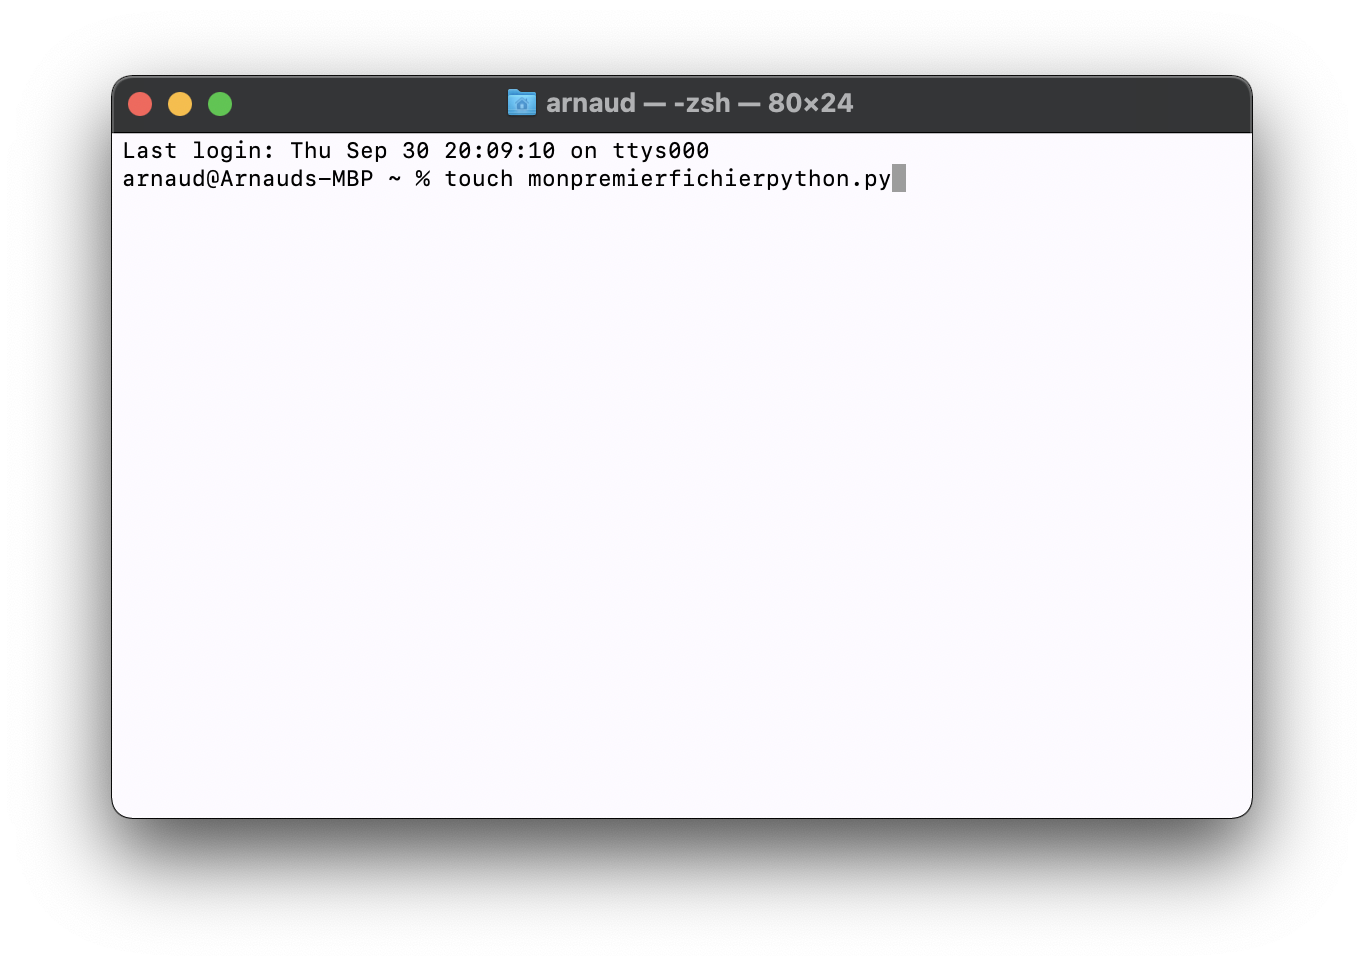
\includegraphics[width=12cm]{1}
\end{center}

\subsection{Création d'un script Python sur Windows}

Pour créer un fichier Python sur Windows, il suffit simplement d'entrer la commande \lstinline{notepad hello.py} dans le bloc-note. Vous pouvez alors simplement l'éditer et l'enregistrer.

\begin{center}
	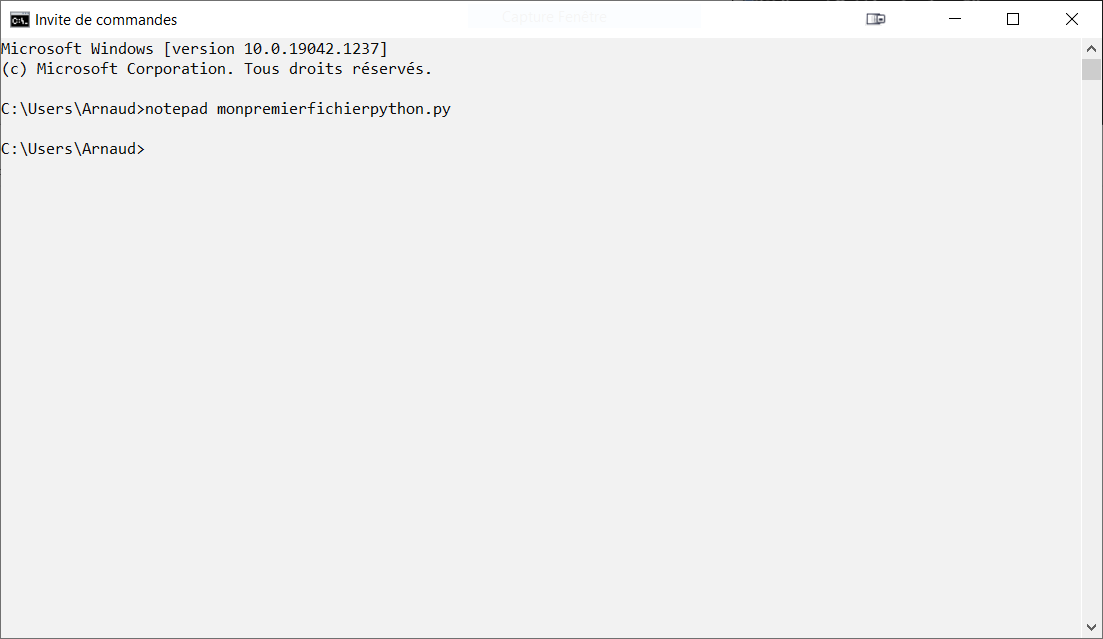
\includegraphics[width=12cm]{4}	
\end{center}

\begin{center}
	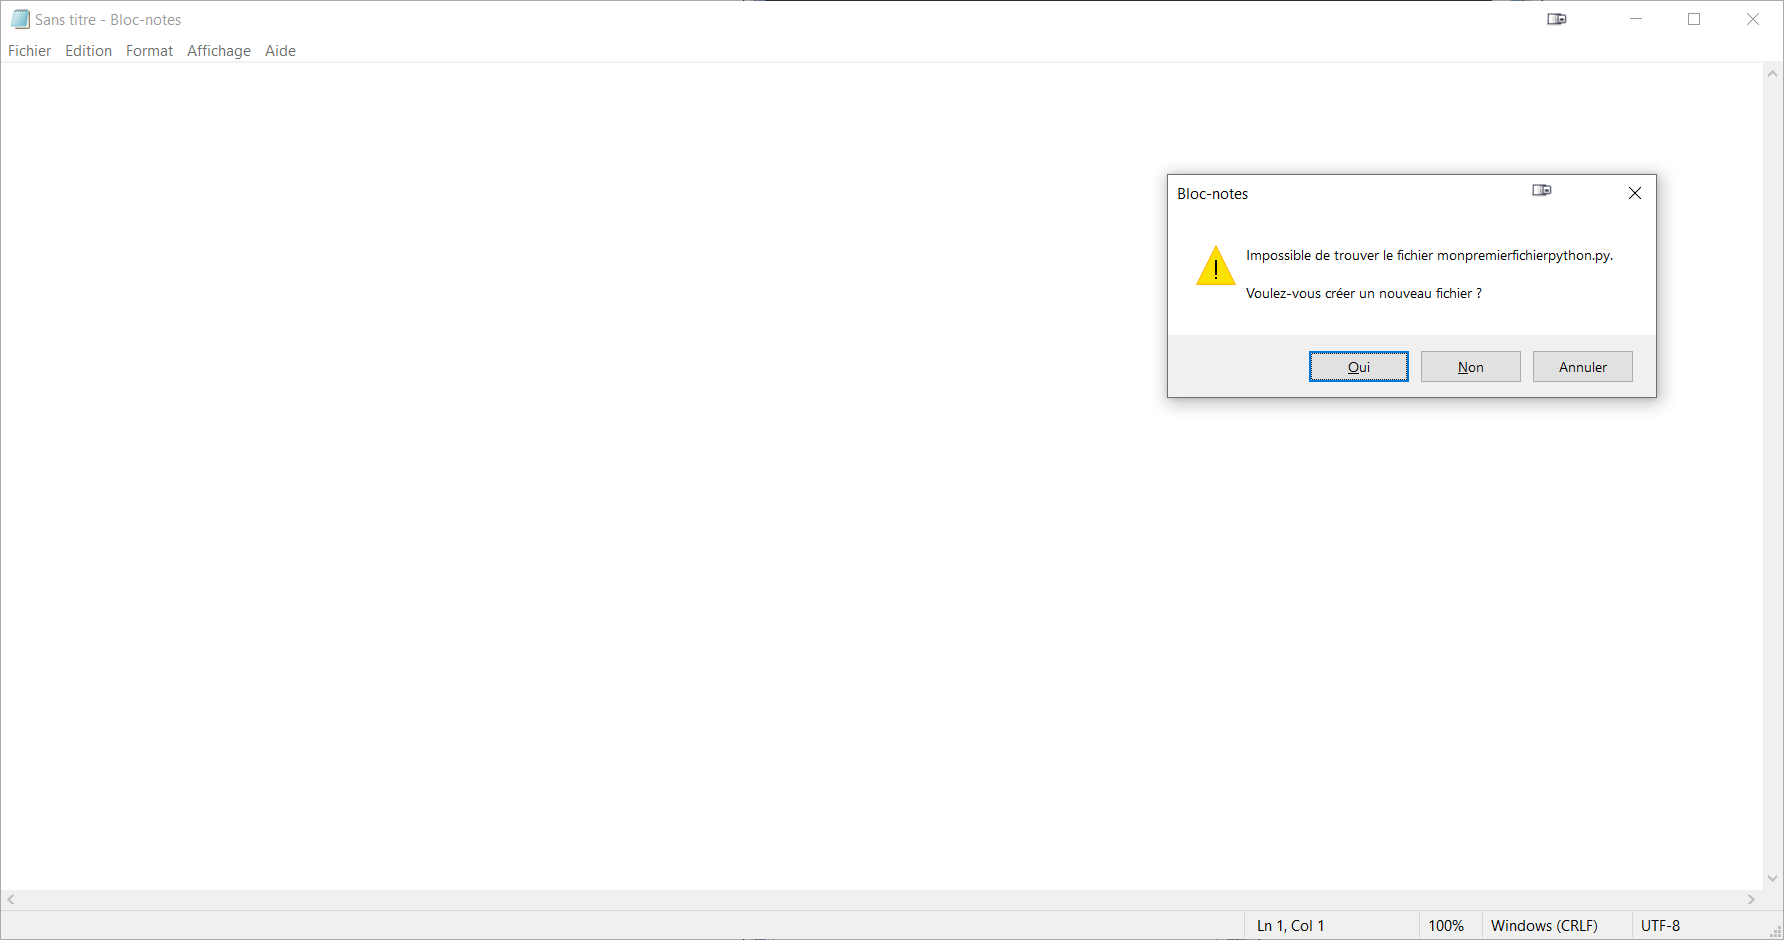
\includegraphics[width=12cm]{5}	
\end{center}

\subsection{IntelliJ IDEA}

Dans le cours, il vous a été demandé d'installer Intellij IDEA, un des l'IDE les plus populaire de ces dernières années. Un IDE (Integrated Developement Environnement) est un programme qui combine différents outils de développement et qui facilite grandement le travail d'un programmeur. La première chose à faire avec le programme est ouvrir et exécuter un script python. Pour ce faire, lancez le programme IntelliJ IDEA et ouvrez le fichier \lstinline{hello.py}.
\begin{center}
	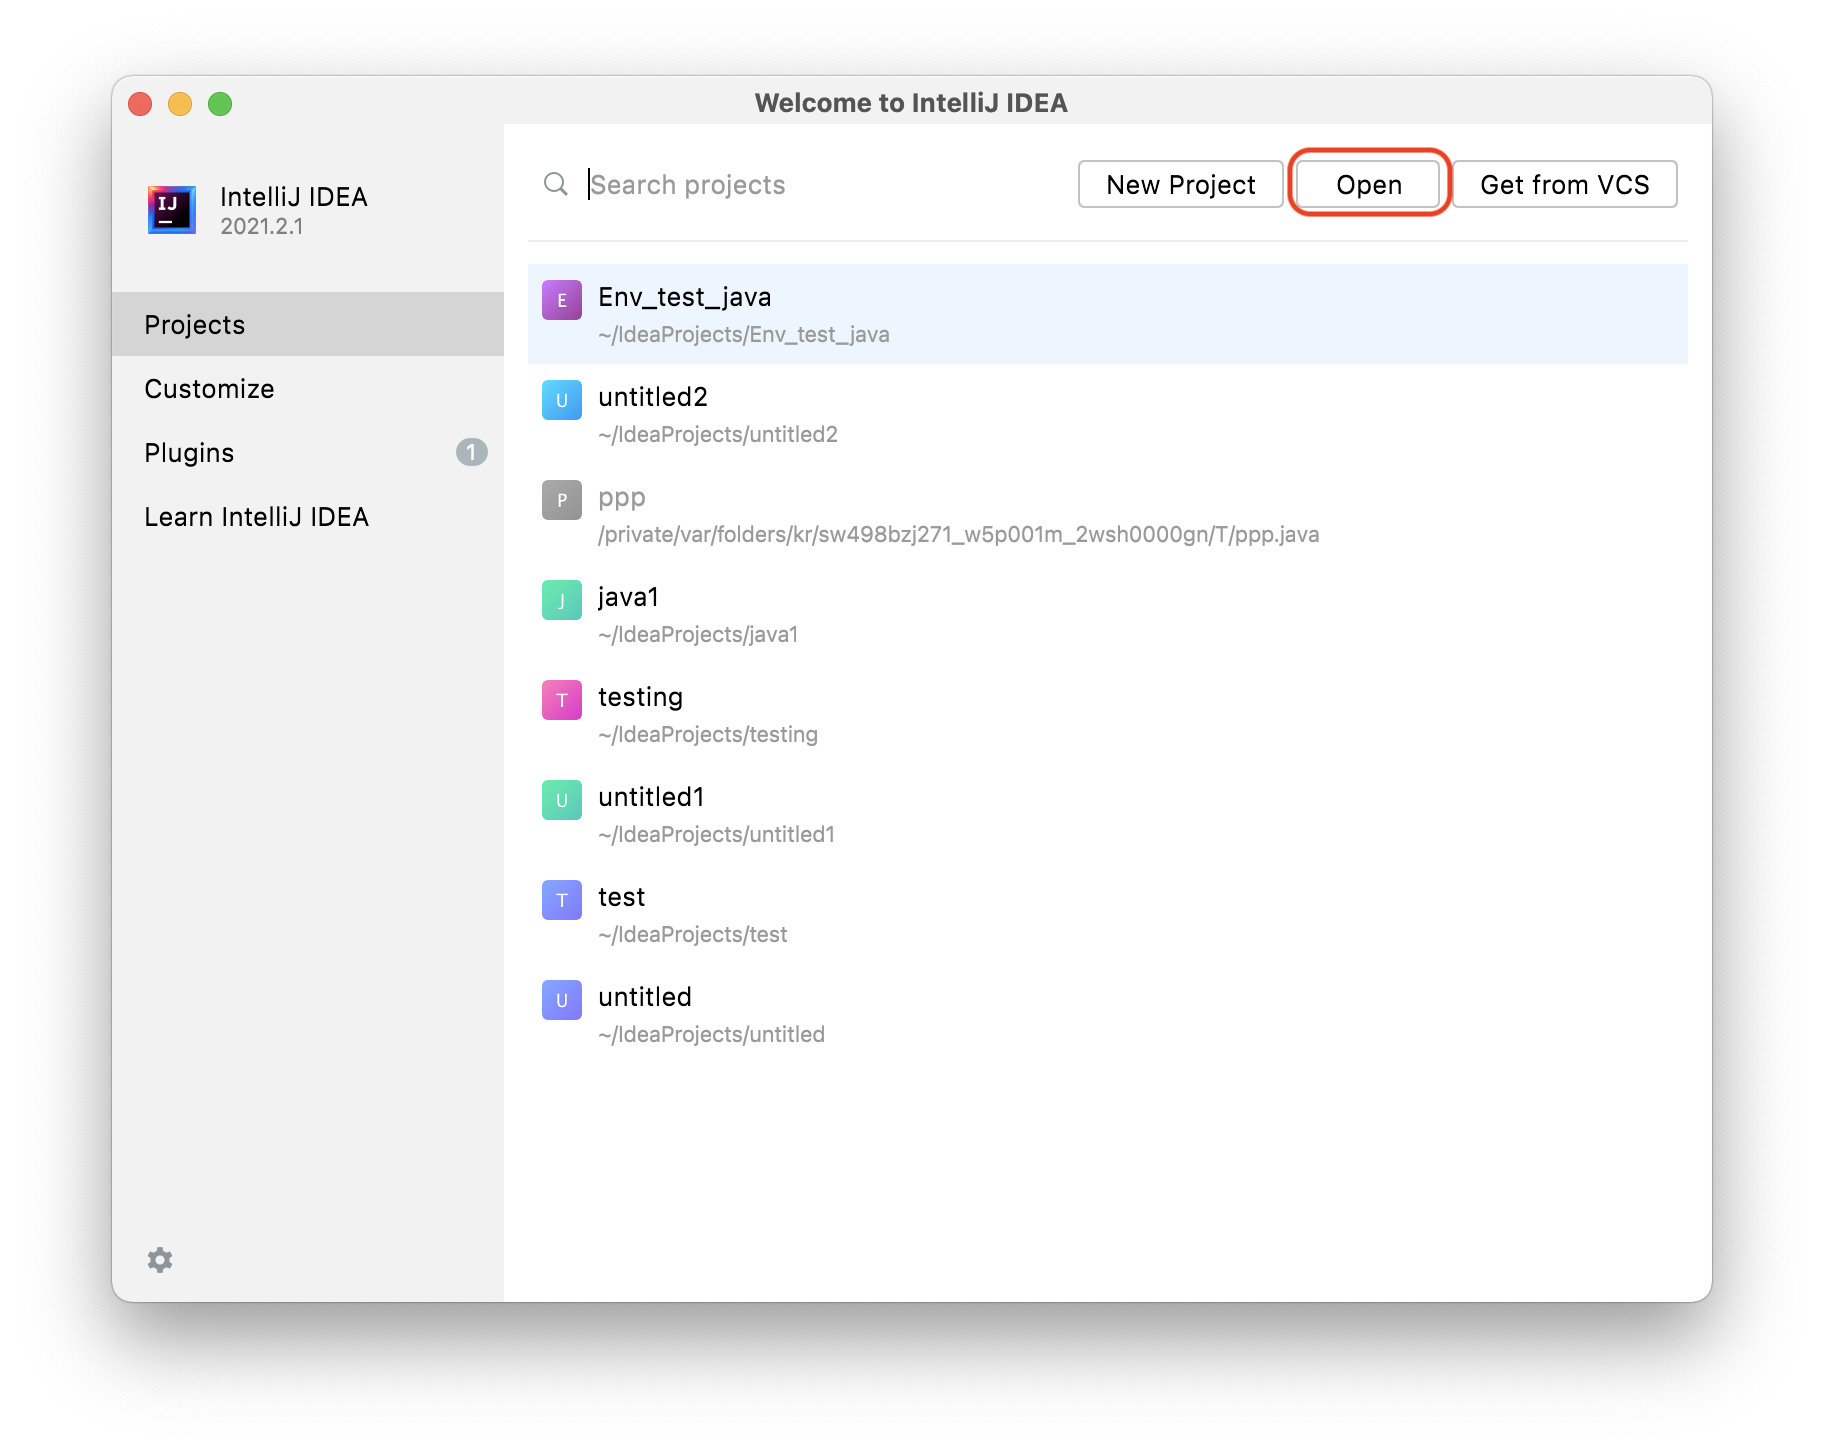
\includegraphics[width=12cm]{2}	
\end{center}

La fenêtre qui vient de s'ouvrir est similaire à un éditeur de texte basique. C'est ici que le code peut être entré et modifié. Notez qu'il est aussi possible de créer directement un fichier depuis votre IDE.
\begin{center}
	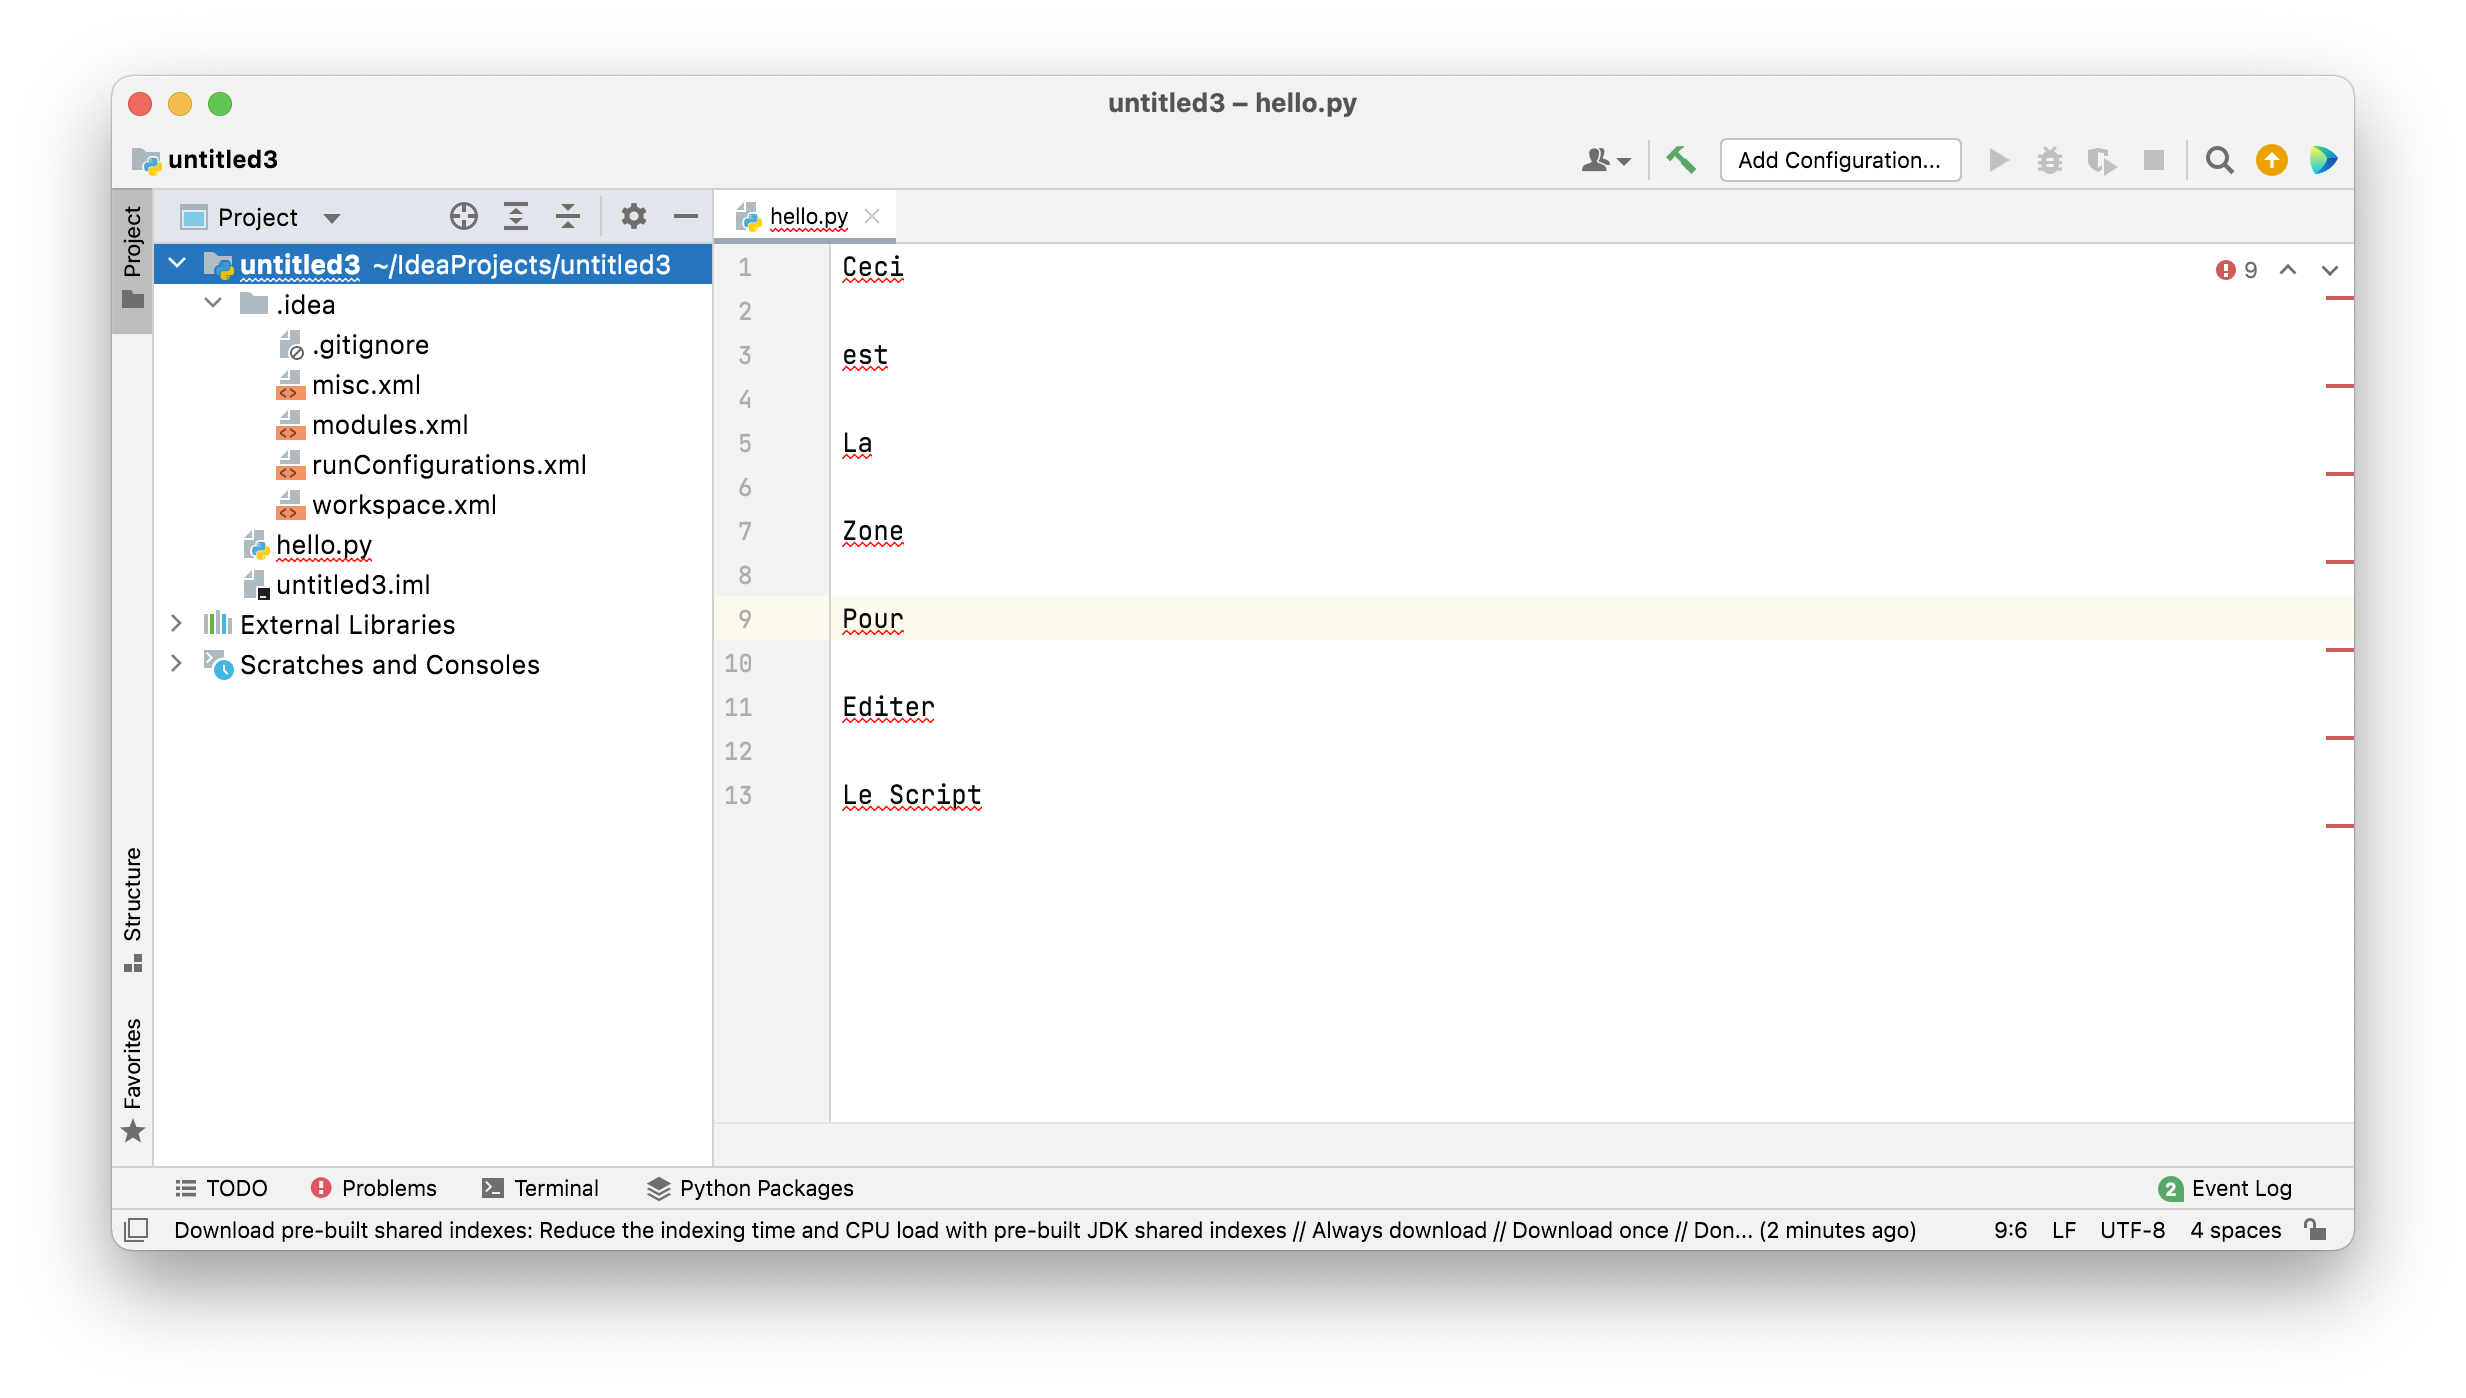
\includegraphics[width=12cm]{3}	
\end{center}


\subsection{Création de variables}

Les variables dans les langages de programmation sont similaires à des noms donnés à une valeur précise.
Pour assigner une valeur à une variable en Python, il suffit de respecter la forme suivante \lstinline{variable=valeur}.

\begin{conseil}
\begin{itemize}
	\item En Python, le type de la variable est défini de façon automatique.
	\item On peut assigner n'importe quelle suite de caractères non-reservée en tant que variable.
	\item Il est aussi possible d'assigner des chaînes de caractères (strings en anglais) ou encore des valeurs booléennes à des variables.
	\item En réassignant une nouvelle valeur à une variable déjà définie, la valeur de la variable va être écrasée et remplacée par la nouvelle valeur.
	\item Plusieurs variables peuvent avoir la même valeur.
\end{itemize}
\end{conseil}


Si vous ouvrez et exécutez le script Python \lstinline{variables.py} (se trouvant sur Moodle, dans le dossier Ressources) qui contient quelques exemples d'attribution de variables, vous pourrez observer comment vous pouvez créer différentes variables mais aussi comment le programme les traite.

\begin{center}
	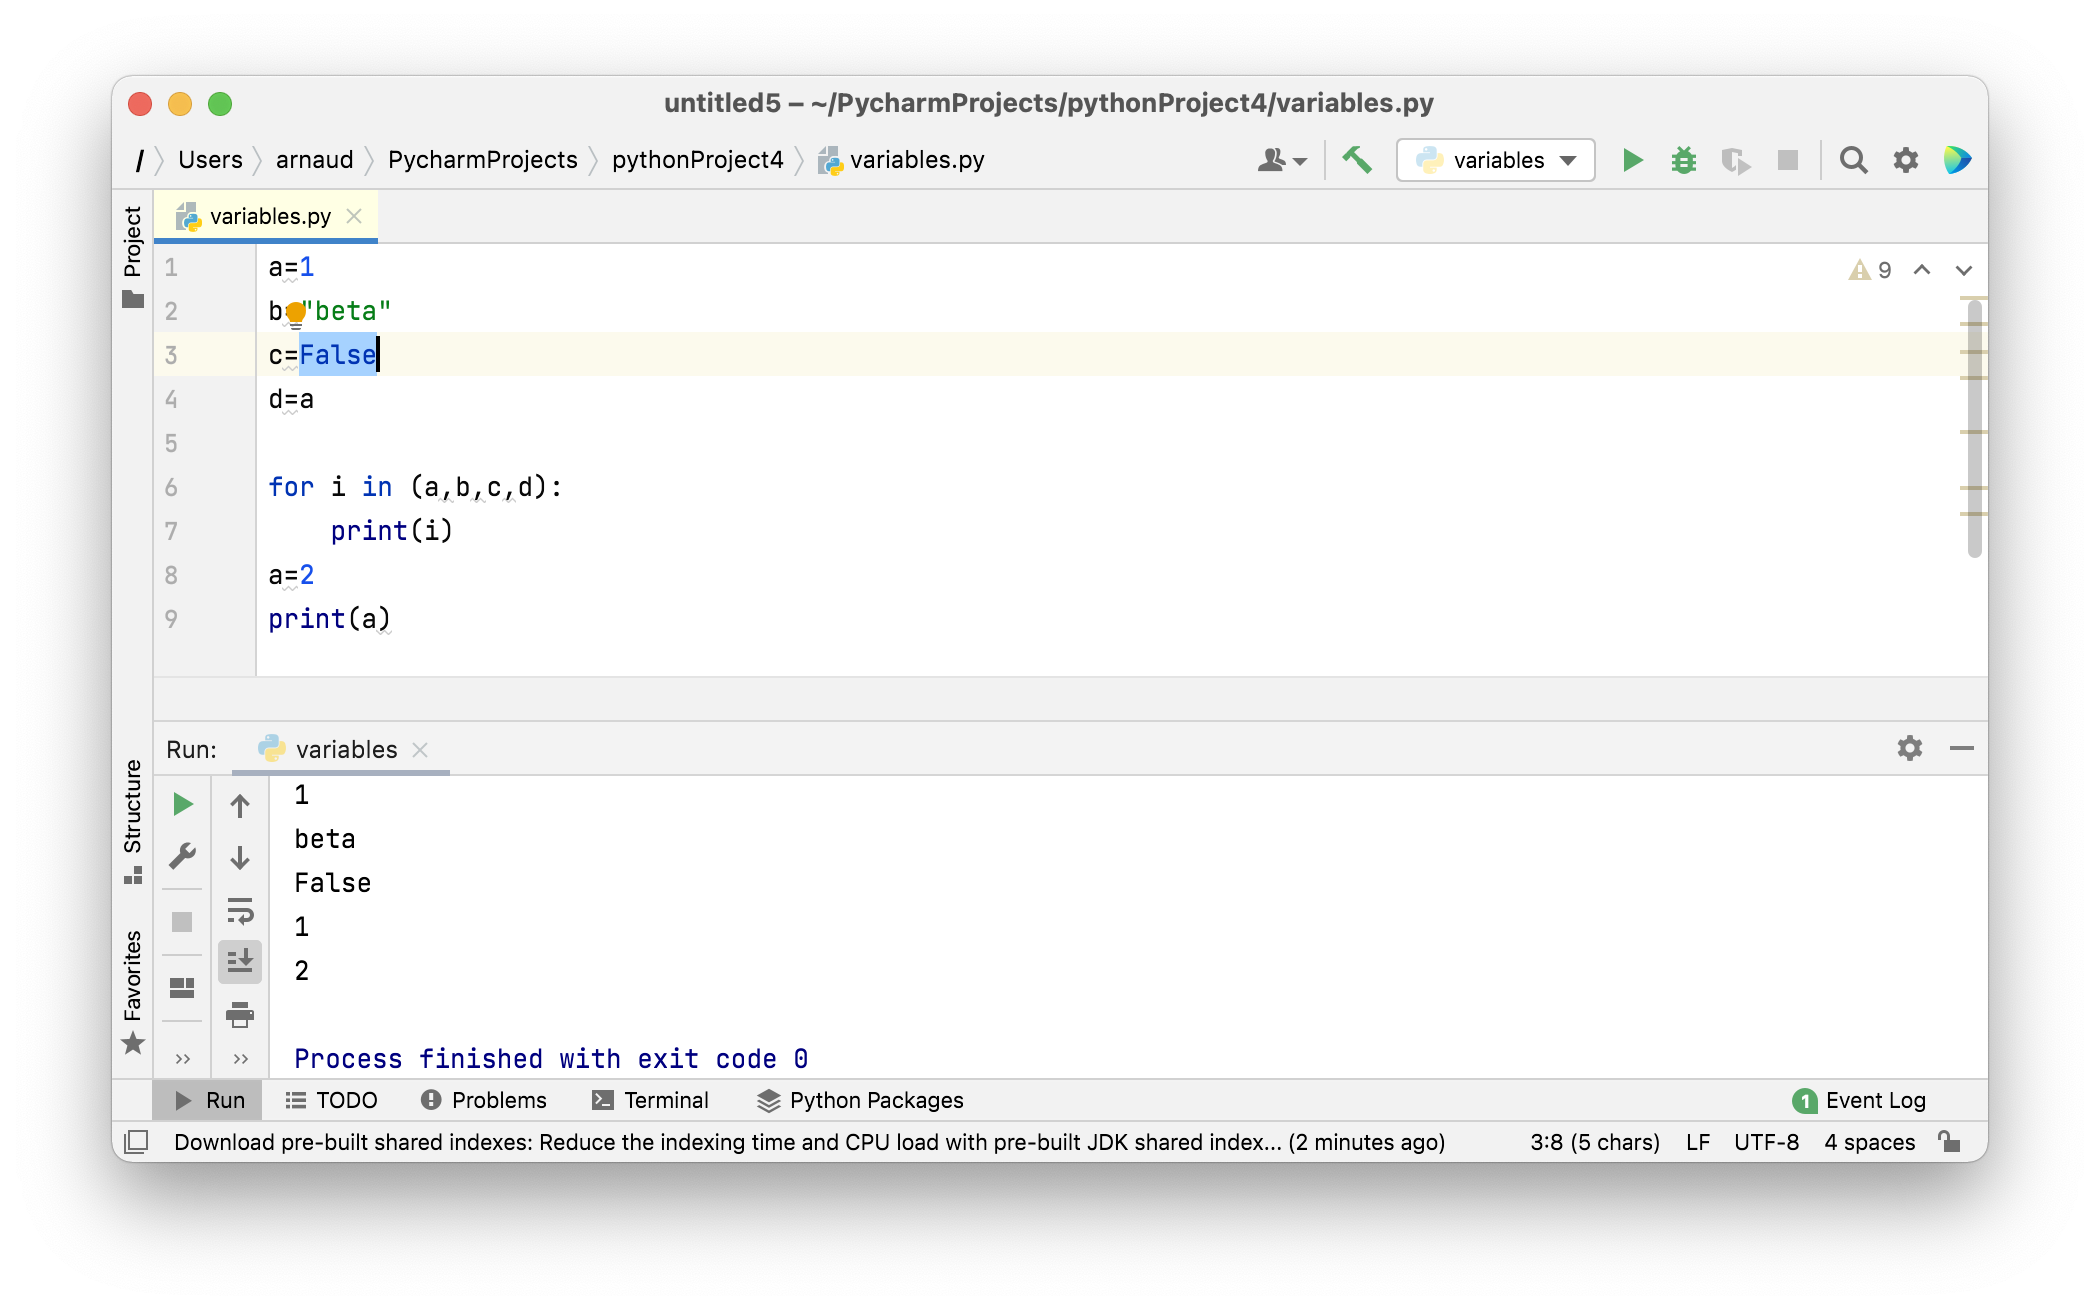
\includegraphics[width=12cm]{6}	
\end{center}


\subsection{L'indentation}

Python est un langage de programmation sensible aux erreurs d'indentation. Une indentation correspond à une tabulation ou un espace. Il sera donc important de bien comprendre comment celles-ci fonctionnent. Prenons par exemple une simple boucle \lstinline{for} qui sera traitée un peu plus loin dans ce guide.\\

Si vous ouvrez et exécutez les deux scripts Python \lstinline{indent1.py} et \lstinline{indent2.py} en allant sur le barre de menu (tout en haut) et en cliquant sur \lstinline{Run > Run `hello'}, vous vous rendrez compte que l'un des deux produit une erreur alors que l'autre fonctionne correctement. En effet, dans un des scripts, la console produit une erreur d'indentation. Après une boucle \lstinline{for}, il est nécessaire de bien respecter l'indentation pour définir son utilité. L'indentation est importante dans la syntaxe d'un script Python. Une erreur d'indentation peut changer le fonctionnement d'un script ou tout simplement empêcher celui-ci de s'exécuter.



\begin{center}	
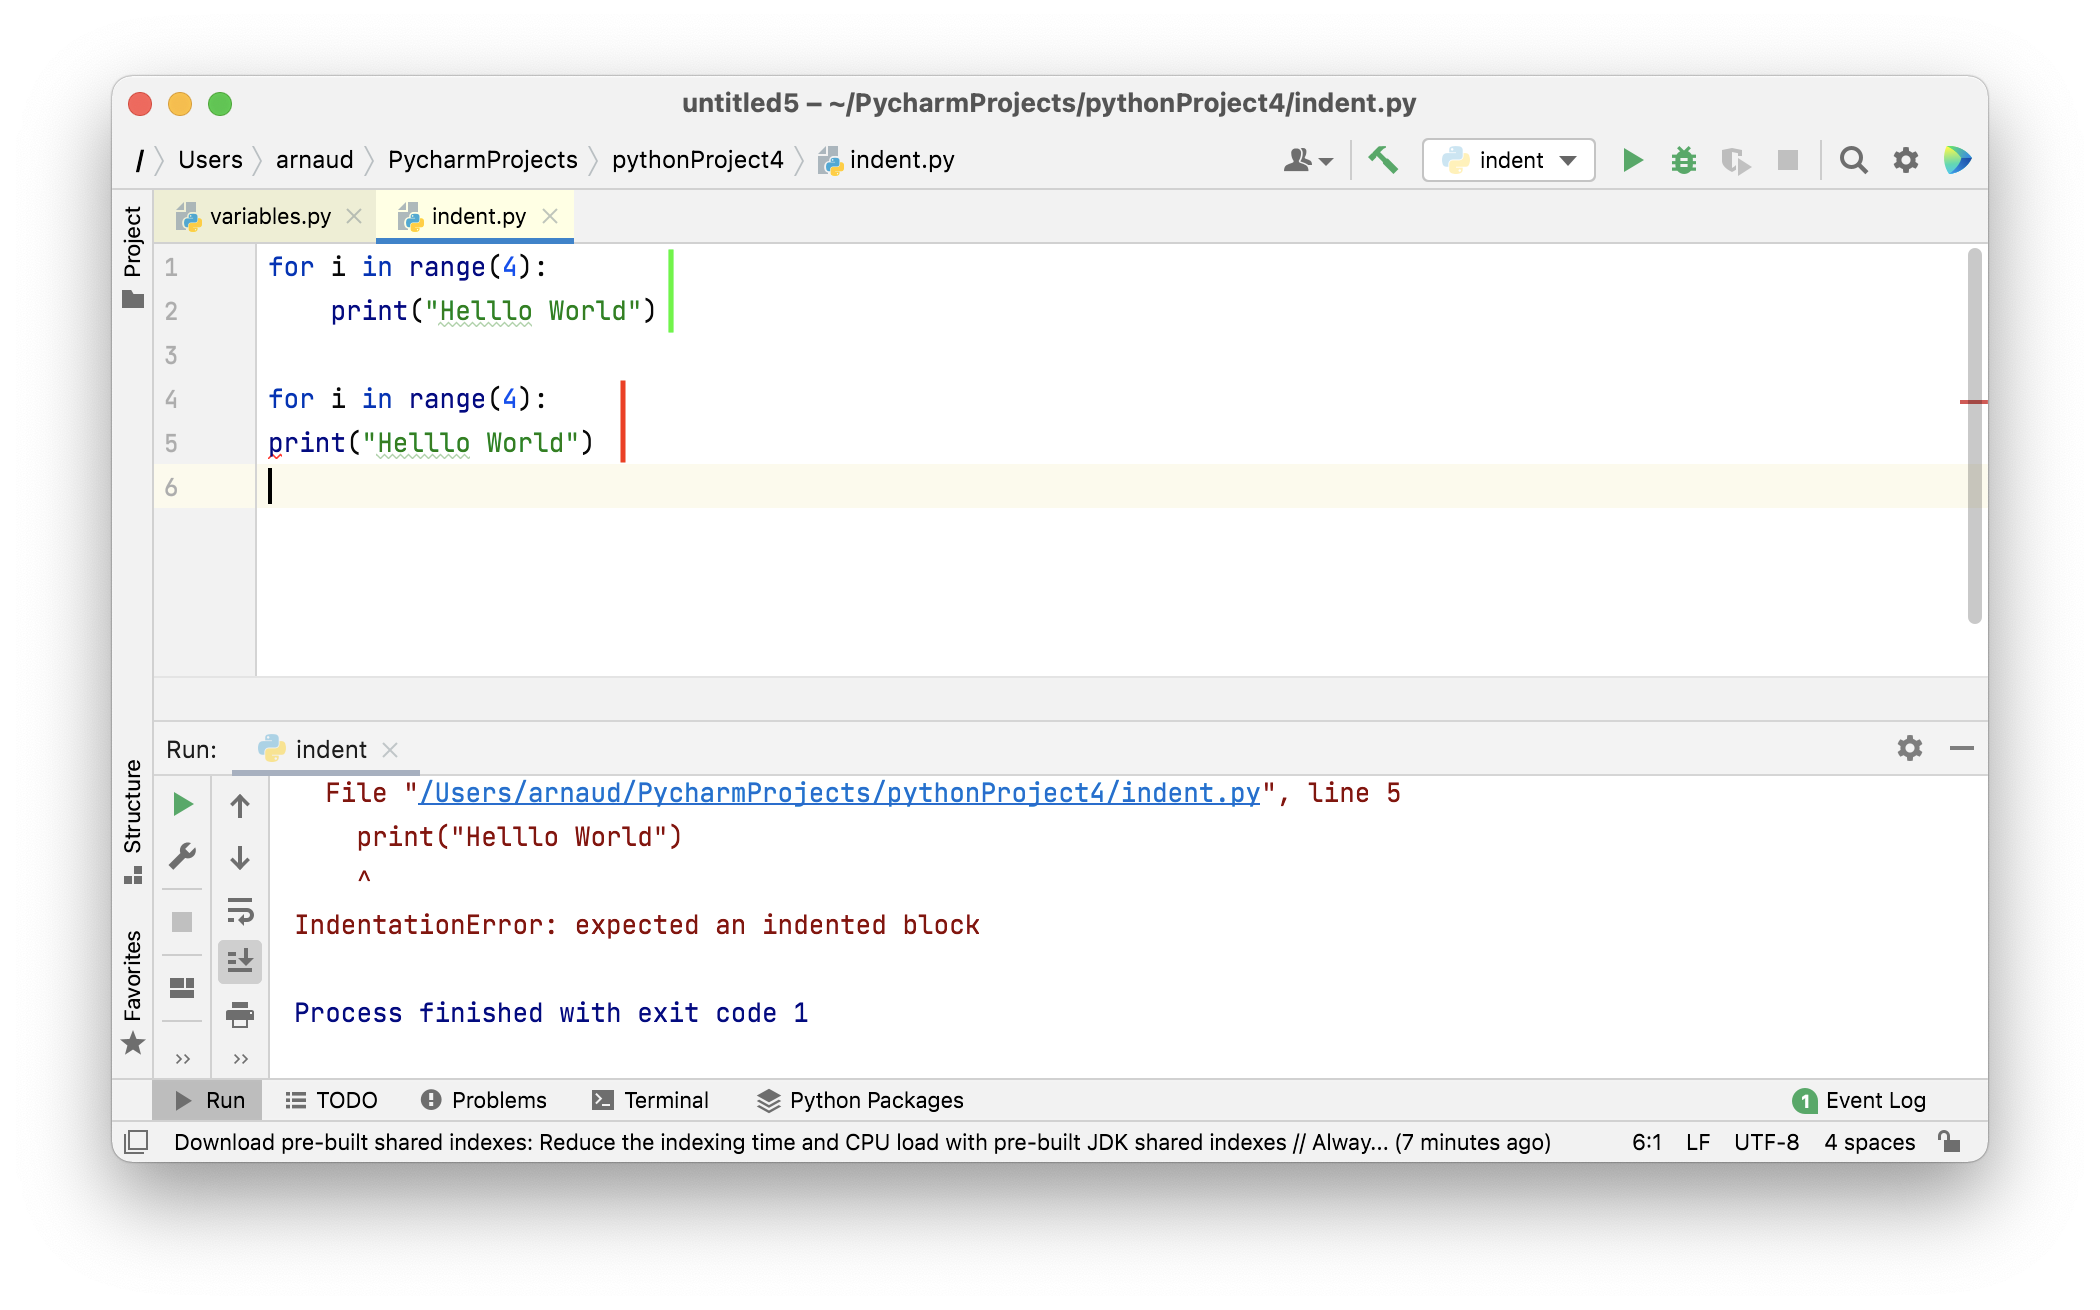
\includegraphics[width=12cm]{7}	
\end{center}


\subsection{Les fonctions}

Dans les langages de programmation, on retrouve un très grand nombre de fonctions. Ces fonctions sont des blocs de code qui, lorsqu'ils sont invoqués avec certains paramètres, effectuent certaines actions. Une des fonctions basique et plutôt importante en Python est la fonction \textbf{print()}.  Cette fonction permet d'afficher à l'écran le contenu de la parenthèse.\\ 
Si vous entrez la ligne de code \lstinline{print("Votremessage")} et que vous exécutez le script, IntelliJ IDEA va vous afficher une ligne de texte. Le message qui apparaît est celui que vous avez entré entre guillemets (à la place de "Votremessage"). C'est le but d'une fonction \lstinline{print()}.
\begin{center}
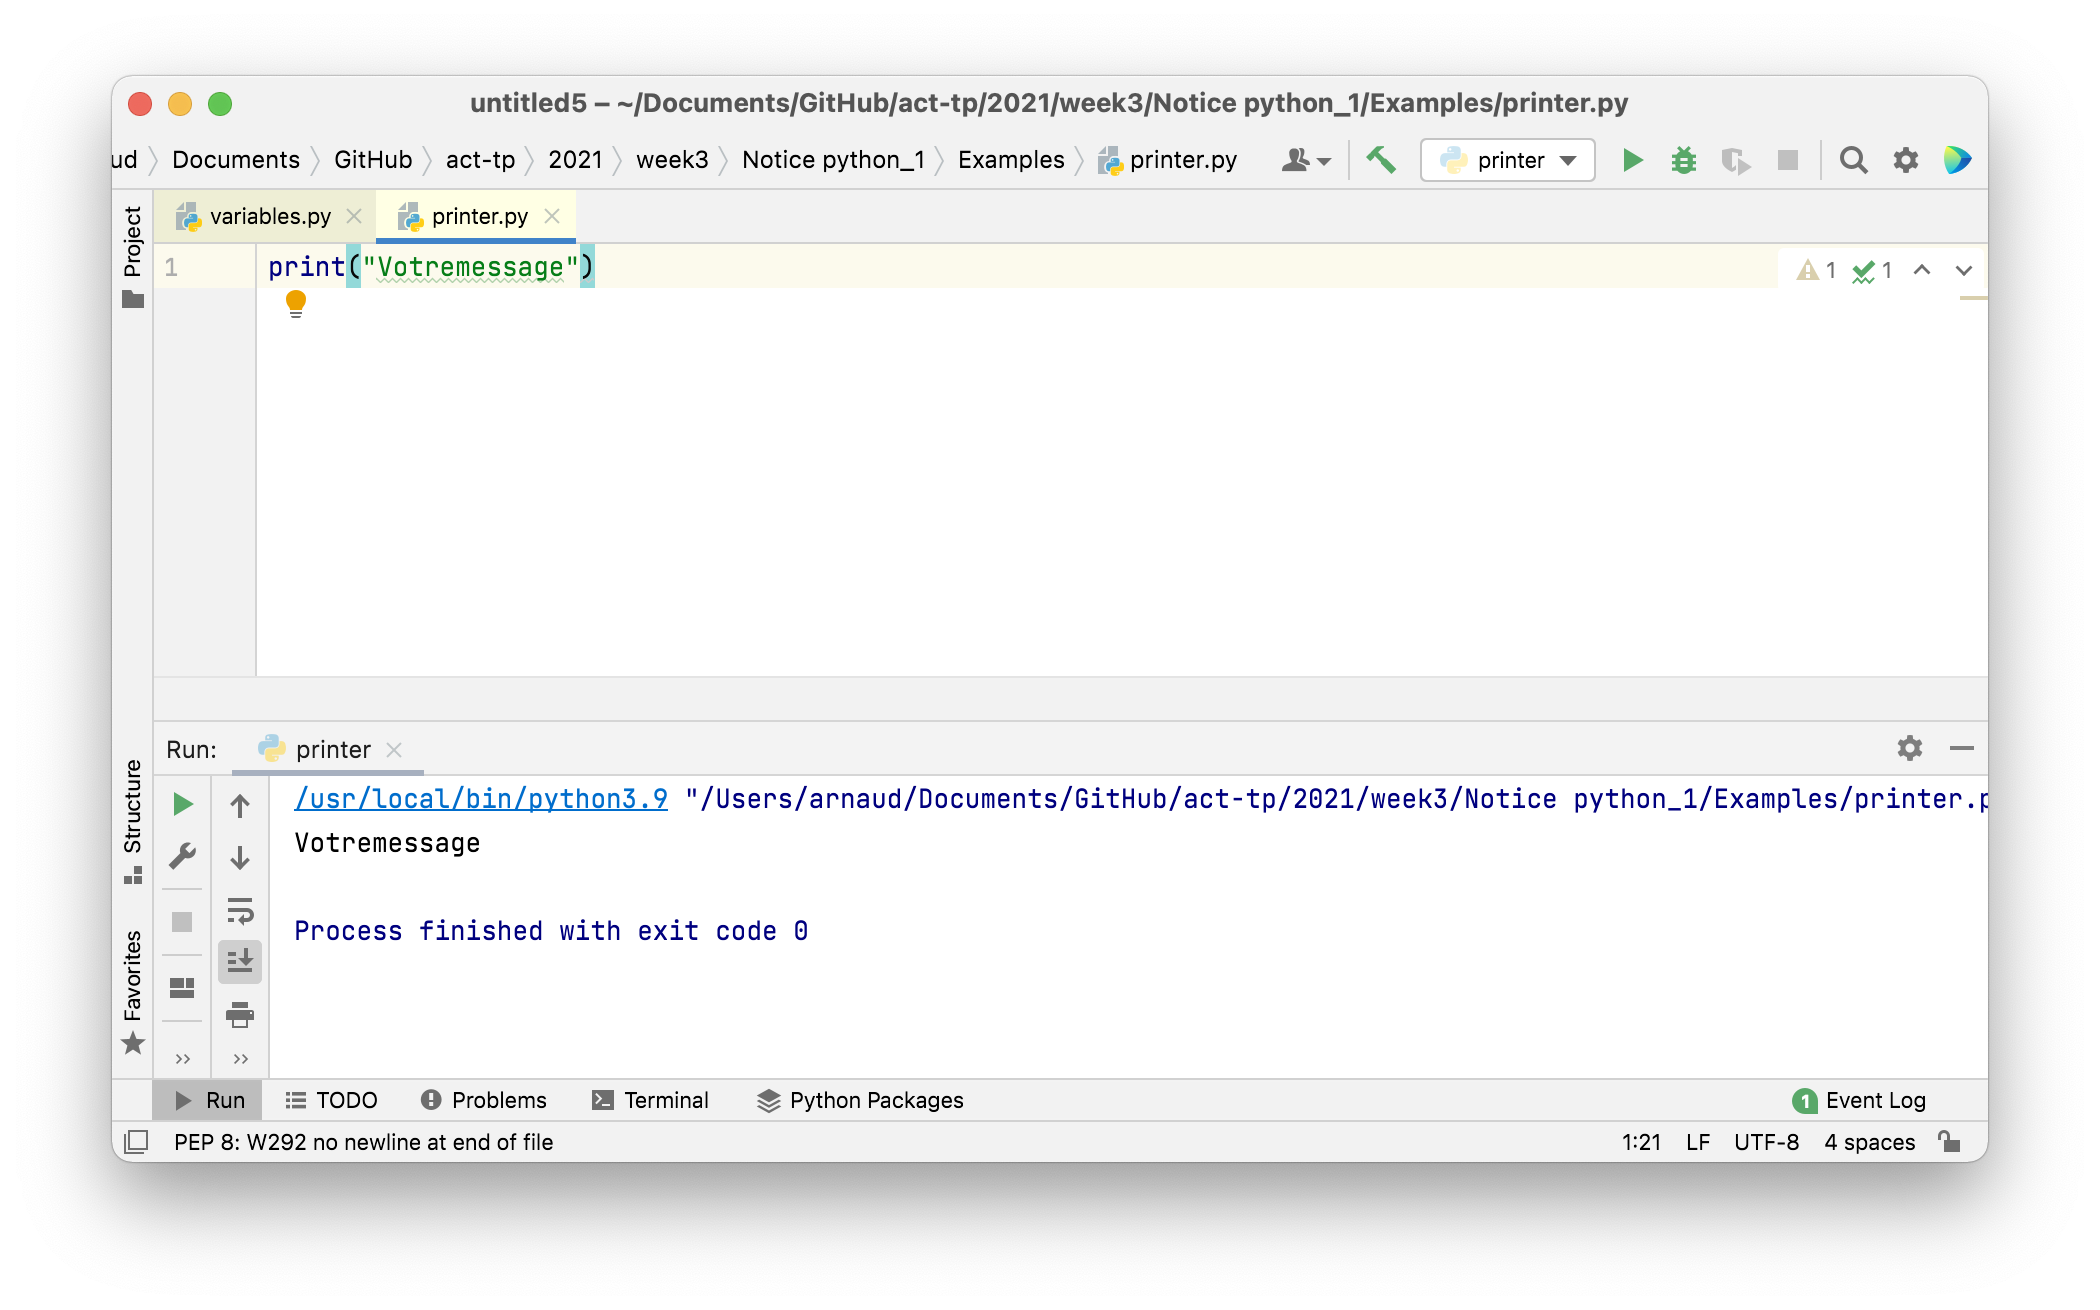
\includegraphics[width=12cm]{8}	
\end{center}


En plus des fonctions incluses dans les librairies Python, il est possible de créer des fonctions complètement personnalisées (généralement plusieurs fonctions sont réunies en une seule) au moyen de la fonction \lstinline{def nomdelafonction():} et de l'utiliser à n'importe quel moment en l'invoquant avec \lstinline{nomdelafonction()}.


Si vous ouvrez et exécutez le script python \lstinline{Arbre.py} (se trouvant sur Moodle, dans le dossier Exercices (version hors ligne)/Code), vous pourrez voir l'exemple de la fonction personnalisée \lstinline{def build_tree(t, branch_length, shorten_by, angle)} qui permet de dessiner un arbre à l'aide d'un algorithme. Nous verrons plus tard dans ce cours comment fonctionnent ces algorithmes.

\begin{center}
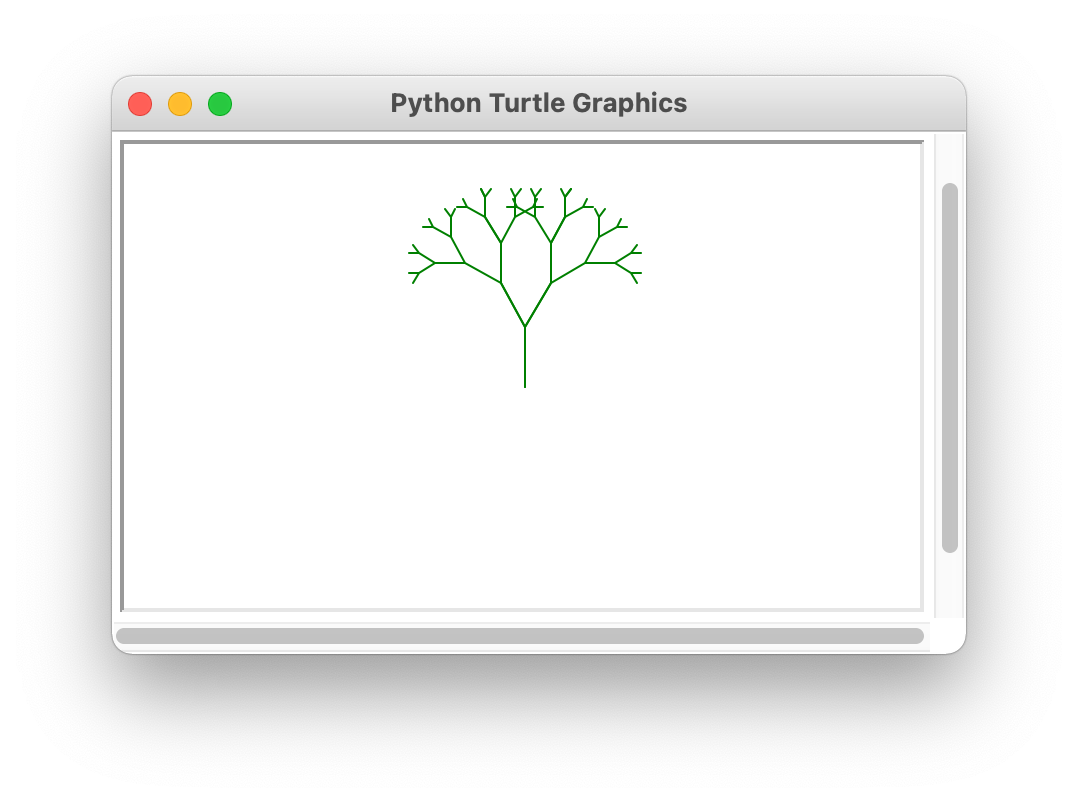
\includegraphics[width=12cm]{arbre.png}		
\end{center}

\end{document}
